\documentclass{beamer}
\usetheme{Boadilla}
\setbeamertemplate{caption}[numbered]
\usepackage{ragged2e}
\usepackage{xcolor}
\usepackage{mathtools}
\usepackage{algorithm2e}


\makeatletter
\setbeamertemplate{footline}
{
  \leavevmode
  \hbox{
  \begin{beamercolorbox}[wd=.8\paperwidth,ht=2.25ex,dp=1ex,center]{title in head/foot}
    \usebeamerfont{title in head/foot}\insertshorttitle
  \end{beamercolorbox}%
  \begin{beamercolorbox}[wd=.2\paperwidth,ht=2.25ex,dp=1ex,center]{date in head/foot}
    \insertframenumber{} / \inserttotalframenumber
  \end{beamercolorbox}}%
  \vskip0pt%
}
\makeatother



\title{\textbf{Portfolio Optimization}}
\subtitle{An Application of Convex Optimization}
\author{A project as part of the course:\\"Advanced Topics in Convex Optimization"\\\vspace{0.4cm}}
\institute{Paraskakis Nikolaos, Undergraduate Student\\\vspace{0.4cm}School of Electrical \& Computer Engineering\\Technical University of Crete}
\date{\footnotesize \today}



\AtBeginSection[]
{
  \begin{frame}{Plan} 
    \frametitle{Contents}
    \tableofcontents[sectionstyle=show/hide,subsectionstyle=show/show/hide]
  \end{frame}
}





\begin{document}



\begin{frame}
\titlepage
\end{frame}


\begin{frame}
\frametitle{Outline}
\tableofcontents[sections={1-8}, subsectionstyle=hide]
\end{frame}





\section{Portfolio}








\subsection{Portfolio}

\begin{frame}
\frametitle{\textbf{Portfolio}}

\begin{definition}
\justifying
A \textbf{portfolio} is a collection of financial investments like stocks, bonds, commodities, cash, and cash equivalents, including closed-end funds and exchange traded funds (ETFs).
\end{definition}

\vspace{0.8cm}
\justifying
A portfolio may also contain:
\begin{itemize}
	\item real estate
	\item art
	\item private investments
\end{itemize}


\end{frame}








\subsection{Assets}

\begin{frame}
\frametitle{\textbf{Assets}}

\begin{definition}
\justifying
An \textbf{asset} is a resource with economic value that an individual, corporation, or country owns or controls with the expectation that it will provide a future benefit, i.e. generate cash flow, reduce expenses, or improve sales, regardless of whether it is manufacturing equipment or a patent.
\end{definition}

\vspace{0.8cm}

\justifying
Assets are reported on a company's balance sheet. They are classified as:
\begin{itemize}
	\item current
	\item fixed
	\item financial
	\item intangible
\end{itemize}

\end{frame}





\subsection{Diversification}

\begin{frame}
\frametitle{\textbf{Diversification}}

\begin{definition}
\justifying
\textbf{Diversification} is a risk management strategy that mixes a wide variety of investments within a portfolio. Diversification can be achieved by buying investments in different asset classes, that are in different countries, industries and sizes of companies.
\end{definition}

\vspace{0.4cm}
\justifying
Diversification's achievments:
\begin{itemize}
	\justifying
	\item yielding \textbf{higher long-term returns}
	\item \textbf{decreasing the risk} of any individual holding or security
\end{itemize}

\end{frame}








\subsection{Portfolio Investment}

\begin{frame}
\frametitle{\textbf{Portfolio Investment}}

\begin{definition}
\justifying
A \textbf{portfolio investment} is ownership of a stock, bond, or other financial asset with the expectation that it will earn a return or grow in value over time, or both.
\end{definition}

\vspace{0.6cm}
\justifying
Portfolio investment categories:
\vspace{0.2cm}
\justifying
\begin{itemize}
	\justifying
	\item \textbf{Strategic investment}, i.e. buying financial assets for long-term growth potential or income yield, or both.
	\item \textbf{Tactical approach}, i.e. active buying and selling activity for short-term gains.
\end{itemize}


\end{frame}





\subsection{Portfolio Management}

\begin{frame}
\frametitle{\textbf{Portfolio Management}}

\begin{definition}
\justifying
\textbf{Portfolio management} is the art and science of selecting and overseeing a group of investments that meet the long-term financial objectives and risk tolerance of a client, a company, or an institution.
\end{definition}

\vspace{0.8cm}
\begin{itemize}
	\justifying
	\item \textbf{Active} portfolio management requires strategic investment.
	\item \textbf{Passive} portfolio management requires tactical approach.
\end{itemize}


\end{frame}










\section{Return}








\subsection{Return}

\begin{frame}
\frametitle{\textbf{Return}}

\begin{definition}
\justifying
A \textbf{return}, also known as a financial return, in its simplest terms, is the money made or lost on an investment over some period of time.
\end{definition}

\vspace{0.8cm}
\justifying
A return can be expressed as
\begin{itemize}
	\justifying
	\item the change in dollar value of an investment over time or
	\item a percentage derived from the ratio of profit to investment.
\end{itemize}

\vspace{0.8cm}
\justifying
Returns can also be presented as
\begin{itemize}
	\justifying
	\item net results (after fees, taxes, and inflation) or
	\item gross returns that do not account for anything but the price change.
\end{itemize}


\end{frame}








\subsection{Rate of Return}

\begin{frame}
\frametitle{\textbf{Rate of Return}}

\begin{definition}
\justifying
A \textbf{Rate of Return (RoR)} is the net gain or loss of an investment over a specified time period, expressed as a percentage of the investment's initial cost. When calculating the rate of return, we determine the percentage change from the beginning of the period until the end.
\end{definition}

\vspace{0.4cm}
\begin{block}
\justifying
The formula is:
$$
RoR = \frac{\text{Current value} - \text{Initial value}}{\text{Initial value}} \cdot 100\%
$$
\end{block}

%\vspace{0.4cm}
%\justifying
%This simple rate of return is sometimes called the basic growth rate, or alternatively, return on investment (ROI).

\end{frame}






\subsection{Return on Investment}

\begin{frame}
\frametitle{\textbf{Return on Investment}}

\begin{definition}
\justifying
\textbf{Return on Investment (ROI)} is a performance measure used to evaluate the efficiency or profitability of an investment or compare the efficiency of a number of different investments. ROI tries to directly measure the amount of return on a particular investment, relative to the investments cost.
\end{definition}

%\vspace{0.4cm}
%\justifying
%To calculate ROI, the benefit (or return) of an investment is divided by the cost of the investment. The result is expressed as a percentage or a ratio.

\vspace{0.4cm}
\begin{block}
\justifying
The formula is:
$$
ROI = \frac{\text{Current Value of Investment} - \text{Cost of Investment}}{\text{Cost of Investment}}
$$
\end{block}

\end{frame}







\subsection{Risk-Adjusted Return}

\begin{frame}
\frametitle{\textbf{Risk-Adjusted Return}}

\begin{definition}
\justifying
A \textbf{risk-adjusted return} is a calculation of the profit or potential profit from an investment that takes into account the degree of risk that must be accepted in order to achieve it. The risk is measured in comparison to that of a virtually risk-free investment.
\end{definition}

\vspace{0.8cm}
\justifying
Risk-adjusted returns are applied to:
\begin{itemize}
	\item individual stocks
	\item investment funds
	\item entire portfolios
\end{itemize}

\end{frame}










\section{Risk}









\subsection{Risk}

\begin{frame}
\frametitle{\textbf{Risk}}

\begin{definition}
\justifying
Risk is defined in financial terms as the chance that an outcome or investment's actual gains will differ from an expected outcome or return.
\end{definition}

\vspace{0.6cm}
\justifying
\begin{itemize}
	\justifying
	\item It includes the possibility of losing some or all of an original investment.
	\item It is assessed by considering historical behaviors and outcomes.
\end{itemize}

\end{frame}







\subsection{Volatility}

\begin{frame}
\frametitle{\textbf{Volatility}}

\begin{definition}
\justifying
\textbf{Volatility} is a statistical measure of the dispersion of returns for a given security or market index. The higher the volatility, the riskier the security. It is often measured from either the standard deviation or variance between returns from that same security or market index.
\end{definition}

\vspace{0.4cm}
\justifying
\begin{itemize}
	\justifying
	\item A \textbf{higher volatility} means that a security's value can potentially be spread out over a large range of values in a short time period.
	\item A \textbf{lower volatility} means that a security's value does not fluctuate dramatically, and tends to be more steady.
\end{itemize}

\end{frame}





\subsection{Risk-free terms}

\begin{frame}
\frametitle{\textbf{Risk-free terms}}

\begin{definition}
\justifying
A \textbf{risk-free asset} is one that has a certain future return and virtually no possibility they will drop in value or become worthless altogether. Risk-free assets tend to have low rates of return, since their safety means investors don't need to be compensated for taking a chance.
\end{definition}

\begin{definition}
\justifying
\textbf{Risk-free return} is the theoretical return attributed to an investment that provides a guaranteed return with zero risks.
\end{definition}

\begin{definition}
\justifying
The \textbf{risk-free rate of return} is the theoretical rate of return of an investment with zero risk.  The risk-free rate of return represents the interest on an investor's money that would be expected from an absolutely risk-free investment over a specified period of time.
\end{definition}

\end{frame}





\subsection{Risk Managemnet}

\begin{frame}
\frametitle{\textbf{Risk Management}}

\begin{definition}
\justifying
\textbf{Risk Management} is a crucial process used to make investment decisions. Risk management involves identifying and analyzing risk in an investment and deciding whether or not to accept that risk given the expected returns for the investment. Some common measurements of risk include standard deviation, Sharpe ratio, beta, value at risk (VaR), conditional value at risk (CVaR), and R-squared.
\end{definition}


\end{frame}







\subsection{Sharpe ratio}

\begin{frame}
\frametitle{\textbf{Sharpe ratio}}

%\justifying
%The Sharpe ratio was developed by Nobel laureate William F. Sharpe and is used to help investors understand the return of an investment compared to its risk.

\vspace{0.6cm}
\begin{definition}
\justifying
The \textbf{Sharpe ratio} is the average return earned in excess of the risk-free rate per unit of volatility or total risk. It serves as an indicator of whether an investment's return is worth the associated risk. A high Sharpe ratio is good when compared to similar portfolios or funds with lower returns.
\end{definition}

\begin{block}
\justifying
The formula is:
$$
\text{Sharpe ratio} = \frac{R_{p} - R_{f}}{\sigma_{p}}
$$
\end{block}

\vspace{0.2cm}
\justifying
where

\vspace{0.2cm}
\justifying
$R_{p}$ : Rate of return of the portfolio\\
$R_{f}$ : Risk-free rate of return\\
$\sigma_{p}$ : Standard deviation of the portfolio's excess return
%\vspace{0.6cm}
%\justifying
%It is a ratio that compares the return specific to an investment with the associated level of volatility an investor is required to assume for holding the investment.


\end{frame}





\section{Modern Portfolio Theory}










\subsection{Introduction}

\begin{frame}
\frametitle{\textbf{Introduction}}

\justifying
\textbf{Modern Portfolio Theory (MPT)} or mean variance portfolio optimization assumes that all investors are risk averse. Hence they would prefer:
\begin{itemize}
	\item a high return portfolio over a low return one for a given level of risk
	\item a low risk portfolio over a high risk one for a given level of return
\end{itemize}

\vspace{0.8cm}
\justifying
This theory states that:
\begin{itemize}
	\item adding assets to a diversified portfolio that have low correlations can decrease portfolio risk without sacrificing return
	\item adding diversification should increase the Sharpe ratio, compared to similar portfolios with a lower level of diversification
\end{itemize}

\end{frame}



\begin{frame}

\justifying
Investors can achieve their best results by choosing an \textbf{optimal mix} of return and risk based on an assessment of their individual tolerance to risk.

\vspace{0.8cm}
\justifying
To choose the best portfolio from a number of possible portfolios two separate decisions need to be made:
\begin{itemize}
	\justifying
	\item Determination of a set of efficient portfolios
	\item Selection of the best portfolio out of the efficient set
\end{itemize}

\end{frame}




\subsection{Determining the efficient set}

\begin{frame}
\frametitle{\textbf{Determining the efficient set}}

\begin{figure}
	\centering
	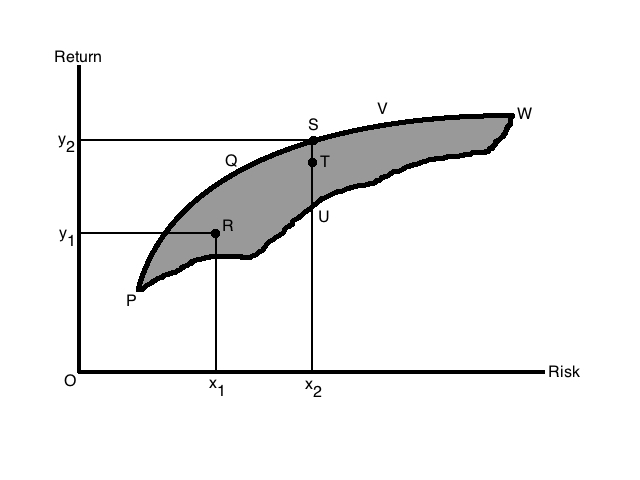
\includegraphics[scale = 0.25]{fig1.jpg}
	\vskip -1cm
	\caption{Risk-return figure of possible portfolios}
	\label{fig:fig1}
\end{figure}

\vskip -0.2cm
\justifying
\begin{itemize}
	\justifying
	\item A portfolio that gives maximum return for a given risk, or minimum risk for given return is an \textbf{efficient portfolio}.
	\item In Figure $1$, the shaded area $PVWP$ includes \textbf{all the possible securities} an investor can invest in.
	\item The efficient portfolios for a given risk level are the ones that lie \textbf{on} the boundary of $PQVW$, which is called the \textbf{Efficient Frontier}.
\end{itemize}

\end{frame}

\begin{frame}

\justifying
Portfolios that lie:
\begin{itemize}
	\justifying
	\item  \textbf{below} the Efficient Frontier are not good enough because the return would be lower for the given risk.
	\item to the \textbf{right} of the Efficient Frontier would not be good enough, as there is higher risk for a given rate of return.
\end{itemize}

\vspace{0.8cm}
\justifying
The Efficient Frontier graphically depicts the benefit of \textbf{diversification} and its curvature shows the relation between portfolio's risk and reward profile.

\end{frame}




\subsection{Choosing the best portfolio}

\begin{frame}
\frametitle{\textbf{Choosing the best portfolio}}

\justifying
For selection of the optimal portfolio or the best portfolio, the risk-return preferences are analyzed.
\vspace{0.4cm}
\begin{itemize}
	\justifying
	\item An investor who is \textbf{highly} risk averse will hold a portfolio on the \textbf{lower left} hand of the frontier.
	\item An investor who is \textbf{not} too risk averse will choose a portfolio on the \textbf{upper} portion of the frontier.
\end{itemize}

\end{frame}

%An investor might have satisfaction represented by $C_2$, but if their satisfaction/utility increases, the investor then moves to curve $C_3$. Thus, at any point of time, an investor will be indifferent between combinations $S_1$ and $S_2$, or $S_5$ and $S_6$.



\begin{frame}

\begin{figure}
	\centering
	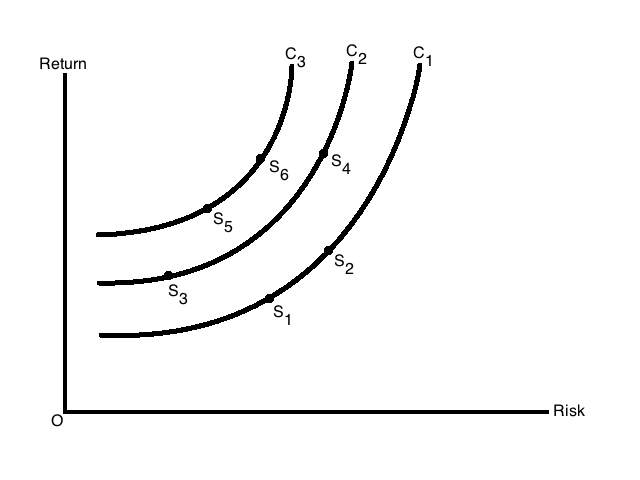
\includegraphics[scale = 0.25]{fig2.jpg}
	\vskip -0.6cm
	\caption{Risk-return indifference curves}
	\label{fig:fig2}
\end{figure}

\vskip -0.2cm
\justifying
\begin{itemize}
	\justifying
	\item Figure $2$ shows the \textbf{risk-return indifference curves} for the investors.
	\item Each of the different points on a particular indifference curve shows a different combination of risk and return, which provide the \textbf{same satisfaction} to the investors.
	\item Each curve to the \textbf{left} represents \textbf{higher} utility or satisfaction and the goal is to maximize the satisfaction.
\end{itemize}

\end{frame}




\begin{frame}

\begin{figure}
	\centering
	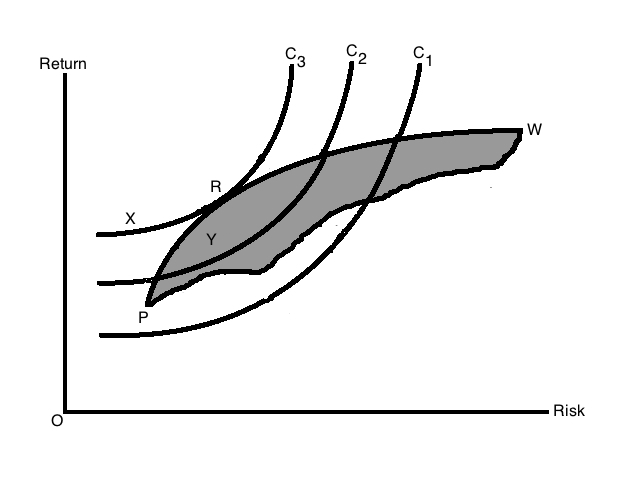
\includegraphics[scale = 0.3]{fig3.jpg}
	\caption{The Efficient Portfolio}
	\label{fig:fig3}
\end{figure}

\justifying
\begin{itemize}
	\justifying
	\item The investor's \textbf{optimal portfolio} is found at the point of \textbf{tangency} of the efficient frontier with the indifference curve.
	\item This point marks the \textbf{highest} level of satisfaction the investor can obtain.
\end{itemize}


\end{frame}



%\begin{frame}


%\justifying
%$R$ is the point where the efficient frontier is tangent to indifference curve $C_3$, and is also an efficient portfolio. With this portfolio, the investor will get highest satisfaction as well as best risk-return combination (a portfolio that provides the highest possible return for a given amount of risk).

%\vspace{0.4cm}
%\justifying
%Any other portfolio, say $X$, is not the optimal portfolio even though it lies on the same indifference curve as it is outside the feasible portfolio available in the market.

%\vspace{0.4cm}
%\justifying
%Portfolio $Y$ is also not optimal as it does not lie on the best feasible indifference curve, even though it is a feasible market portfolio. 

%\vspace{0.4cm}
%\justifying
%Another investor having other sets of indifference curves might have some different portfolio as their best/optimal portfolio.



%\end{frame}

%\begin{frame}

%\vspace{0.8cm}
%\justifying
%$R_1$ is the risk-free return, or the return from government securities, as those %securities are considered to have no risk for modeling purposes.

%\vspace{0.8cm}
%\justifying
%$R_{1}PX$ is drawn so that it is tangent to the efficient frontier. Any point on the line %$R_{1}PX$ shows a combination of different proportions of risk-free securities and %efficient portfolios.

%\vspace{0.8cm}
%\justifying
%The satisfaction an investor obtains from portfolios on the line $R_{1}PX$ is more than the satisfaction obtained from the portfolio $P$.
%\begin{itemize}
	%\item All portfolio combinations to the left of $P$ show combinations of risky and risk-free assets.
	%\item All portfolio combinations to the right of $P$ represent purchases of risky assets made with funds borrowed at the risk-free rate.
%\end{itemize}

%\end{frame}





%\begin{frame}

%\justifying
%In the case that an investor has invested all their funds, additional funds can be borrowed at risk-free rate and a portfolio combination that lies on $R_{1}PX$ can be obtained. $R_{1}PX$ is known as the Capital Market Line (CML).

%\vspace{0.8cm}
%\justifying
%This line represents the risk-return trade off in the capital market. The CML is an upward sloping line, which means that the investor will take higher risk if the return of the portfolio is also higher.

%\vspace{0.8cm}
%\justifying
%The portfolio $P$ is the most efficient portfolio, as it lies on both the CML and Efficient Frontier, and every investor would prefer to attain this portfolio, $P$. The $P$ portfolio is known as the Market Portfolio and is also the most diversified portfolio. It consists of all shares and other securities in the capital market.

%In the market for portfolios that consists of risky and risk-free securities, the CML represents the equilibrium condition. The Capital Market Line says that the return from a portfolio is the risk-free rate plus risk premium. Risk premium is the product of the market price of risk and the quantity of risk, and the risk is the standard deviation of the portfolio.

%\end{frame}


\subsection{Capital Market Line}

\begin{frame}
\frametitle{\textbf{Capital Market Line (CML)}}

\begin{definition}
\justifying
The \textbf{Capital Market Line (CML)} represents portfolios that optimally combine risk and return. It is a theoretical concept that represents all the portfolios that optimally combine the risk-free rate of return and the market portfolio of risky assets.
\end{definition}

\vspace{0.8cm}
\justifying
All investors will choose a position on the Capital Market Line, in equilibrium, by borrowing or lending at the risk-free rate, since this maximizes return for a given level of risk.

\vspace{0.8cm}
\justifying
The \textbf{slope} of the CML is the \textbf{Sharpe ratio} of the market portfolio.

\end{frame}


\begin{frame}

\justifying
The intercept point of CML and Efficient Frontier would result in the most efficient portfolio called the tangency (market) portfolio.

\vspace{0.2cm}
\justifying
As a generalization:
\begin{itemize}
	\justifying
	\item \textbf{buy} assets if Sharpe ratio is \textbf{above} CML
	\item \textbf{sell} assets if Sharpe ratio is \textbf{below} CML
\end{itemize}

\vspace{0.2cm}
\begin{block}
\justifying
The formula is:
$$
R_{p} = R_{f} + \frac{R_{t} - R_{f}}{\sigma_{t}} \sigma_{p}
$$
\end{block}

\vspace{0.2cm}
\justifying
where

\vspace{0.2cm}
\justifying
$R_{p}$ : Rate of return of the portfolio\\
$R_{t}$ : Rate of return of the market portfolio\\
$R_{f}$ : Risk-free rate of return\\
$\sigma_{t}$ : Standard deviation of the market portfolio's excess return\\
$\sigma_{p}$ : Standard deviation of the portfolio's excess return

\end{frame}


\begin{frame}

\begin{figure}
	\centering
	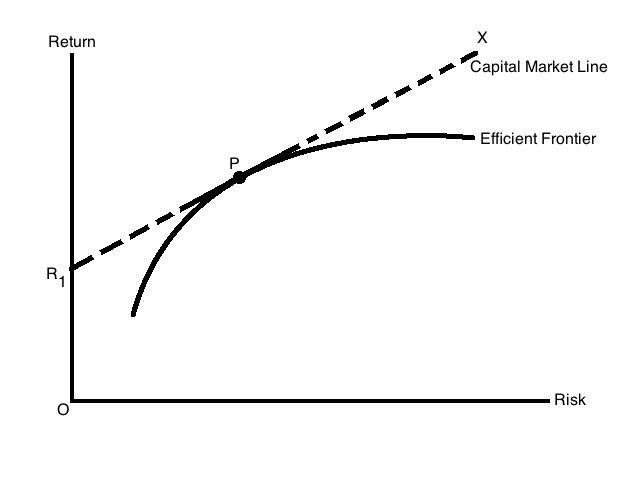
\includegraphics[scale = 0.25]{fig4.jpg}
	\caption{The Combination of Risk-Free Securities with the Efficient Frontier and Capital Market Line (CML)}
	\label{fig:fig4}
\end{figure}

\vskip -0.4cm
\justifying
\begin{itemize}
	\justifying
	\item Portfolios may also include risk-free securities.
	\item A portfolio with risk-free securities will enable an investor to achieve a \textbf{higher} level of satisfaction.
\end{itemize}

\end{frame}



\begin{frame}

The Efficient Frontier represents combinations of risky assets.

\vspace{0.8cm}
\justifying
If we draw a line from the risk-free rate of return, which is \textbf{tangential} to the Efficient Frontier, we get the Capital Market Line. The point of tangency is the \textbf{most efficient} portfolio.

\vspace{0.8cm}
\justifying
Moving:
\begin{itemize}
	\justifying
	\item \textbf{up} the CML will increase portfolio's risk and consequently increase return expectation
	\item \textbf{down} the CML will decrease portfolio's risk and consequently decrease return expectation
\end{itemize}

\end{frame}


%\begin{frame}

%\begin{figure}
	%\centering
	%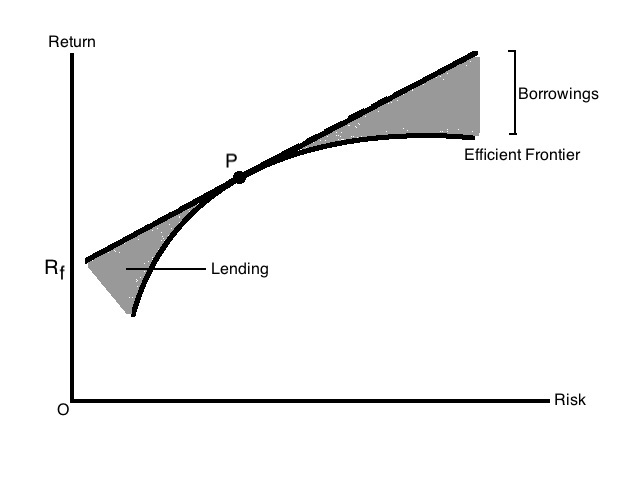
\includegraphics[scale = 0.25]{fig5.jpg}
	%\caption{CML and Risk-Free Lending and Borrowing}
	%\label{fig:fig5}
%\end{figure}

%\justifying
%Figure $5$ shows that an investor will choose a portfolio on the efficient frontier, in the absence of risk-free investments. But when risk-free investments are introduced, the investor can choose the portfolio on the CML (which represents the combination of risky and risk-free investments).

%\end{frame}


%\begin{frame}

%\justifying
%This can be done with borrowing or lending at the risk-free rate of interest ($R_{f}$) and the purchase of efficient portfolio $P$. The portfolio an investor will choose depends on their preference of risk.
%\begin{itemize}
	%\justifying
	%\item The portion from $R_{f}$ to $P$, is investment in risk-free assets and is called Lending Portfolio. In this portion, the investor will lend a portion at risk-free rate.
	%\item The portion beyond $P$ is called Borrowing Portfolio, where the investor borrows some funds at risk-free rate to buy more of portfolio $P$.
%\end{itemize}

%\end{frame}











\section{Optimization Problems}










\subsection{Formulation}

\begin{frame}
\frametitle{\textbf{Formulation}}

\justifying
Let a long only portfolio with $n$ assets. We define the following:

\vspace{0.4cm}
\begin{itemize}
	\justifying
	\item Invest fraction $w_{i}$ in asset $i$ with $i = 1,2, \dots, n$.
	\item Vector $\mathbf{w} \in \mathbb{R}^{n}$ is the portfolio allocation vector.
	\item Long only portfolio means that $w_{i} > 0$ for $i = 1,2, \dots, n$.
	\begin{itemize}
		\justifying
		\item A \textbf{long position} refers to the purchase of an asset with the expectation it will increase in value.
		\item A \textbf{short position} is created when a trader sells a security first with the intention of repurchasing it or covering it later at a lower price.
	\end{itemize}
	\item It must $\mathbf{1}^{T} \mathbf{w} = 1$.
	\item The number of the trading days in a year is considered to be $252$.
\end{itemize}

\end{frame}

\begin{frame}


\begin{itemize}
	\justifying
	\item Vector $\boldsymbol\mu \in \mathbb{R}^{n}$ contains the annual mean returns of each asset.\\
	It is being calculated as follows:
	\begin{itemize}
		\justifying
		\item First, we compute the percentage change on the daily stocks' close prices (the percentage change between each row and its immediately previous row).
		\item Then, we get $\boldsymbol\mu$ as the annualized geometric mean of the percentage changes calculated before.
		\item Let $n$ stocks, data of $m$ days and each percentage change of $i$-th stock's daily price as $r_{i,k}$, $k = 1, \dots, m-1$. The formula for stock $i$ is:\\
	$\boldsymbol\mu_{i} = {\left((1+r_{i,1}) \cdot (1+r_{i,2}) \cdot \ldots \cdot (1+r_{i,m})\right)}^{(\frac{252}{m-1})} - 1$.
	\end{itemize}
\end{itemize}
	
\end{frame}



\begin{frame}


\begin{itemize}
	\justifying
	\item Matrix $\mathbf{\Sigma} \in \mathbb{R}^{n \times n}$ is the annual covariance matrix of portfolio's assets.\\
	It is being calculated as follows:\\
	\begin{itemize}
		\item First, we compute the percentage change on the daily stocks' close prices (the percentage change between each row and its immediately previous row).
		\item Let $n$ stocks, data of $m$ days and each percentage change of $i$-th stock's daily price as $r_{i,k}$, $k = 1, \dots, m-1$. The formula for the covariance between stock $i$ and stock $j$ is:\\
	$Cov(s_i,s_j) = \frac{\sum_{k=1}^{m-1}{(r_{i,k} - \bar{r_{i}})(r_{j,k} - \bar{r_{j}})}}{m-1}$
	\end{itemize}
\end{itemize}
	
\end{frame}




\begin{frame}


\begin{itemize}
	\justifying
	\item Portfolio's annual variance is given by $\mathbf{w}^{T}\mathbf{\Sigma}\mathbf{w}$.
	\item Given that portfolio's volatility {risk} is defined as the square root of portfolio's variance, then minimization on the portfolio's volatility is equivalent to minimization on the portfolio's variance.
	\vspace{0.2cm}
	\item Portfolio's annual return is given by $\boldsymbol\mu^{T} \mathbf{w}$.
	\vspace{0.2cm}
	\item Quadratic utility is given by $\boldsymbol\mu^{T} \mathbf{w} - \gamma \frac{1}{2}\mathbf{w}^{T}\mathbf{\Sigma}\mathbf{w}$ where $\gamma$ is the risk aversion parameter.
	\vspace{0.2cm}
	\item Risk-free rate of return is equal to zero.
\end{itemize}



\end{frame}





\subsection{Minimum volatility}

\begin{frame}
\frametitle{\textbf{Minimum volatility}}

\justifying
Let a portfolio as initially described above. We want to obtain the optimal vector $\mathbf{w}$ that minimizes portfolio's volatility (risk). To do so, we have to solve the following convex optimization problem:

\vspace{0.2cm}
\justifying
\begin{equation}
\begin{aligned}
\label{eq:1}
\min_{\mathbf{w}} \quad & \frac{1}{2}\mathbf{w}^{T}\mathbf{\Sigma}\mathbf{w} \\
\textrm{s.t.} \quad & \mathbf{1}^{T} \mathbf{w} = 1 \\
                             & 0 \leq w_{i} \leq 1 \textrm{ , } i = 1, 2, \dots n \\
\end{aligned}
\end{equation}

\end{frame}





\subsection{Minimum volatility for a given target return}

\begin{frame}
\frametitle{\textbf{Minimum volatility for a given target return}}

\justifying
Let a portfolio as initially described above. We want to obtain the optimal vector $\mathbf{w}$ that minimizes portfolio's volatility (risk) and gives annual portfolio's return $r$. To do so, we have to solve the following convex optimization problem:

\vspace{0.2cm}
\justifying
\begin{equation}
\begin{aligned}
\label{eq:2}
\min_{\mathbf{w}} \quad & \frac{1}{2}\mathbf{w}^{T}\mathbf{\Sigma}\mathbf{w} \\
\textrm{s.t.} \quad & \boldsymbol\mu^{T} \mathbf{w} = r \\
                             & \mathbf{1}^{T} \mathbf{w} = 1 \\
                             & 0 \leq w_{i} \leq 1 \textrm{ , } i = 1, 2, \dots n \\
\end{aligned}
\end{equation}


\vspace{0.2cm}
\justifying
By problem's nature, we can easily see that constraint $\boldsymbol\mu^{T} \mathbf{w} = r$ is equivalent to constraint $\boldsymbol\mu^{T} \mathbf{w} \geq r$.

\end{frame}






\subsection{Maximum return for a given target volatility}

\begin{frame}
\frametitle{\textbf{Maximum return for a given target volatility}}

\justifying
Let a portfolio as initially described above. We want to obtain the optimal vector $\mathbf{w}$ that maximizes portfolio's return and gives annual portfolio's volatility (risk) $v$. Note that maximizing $\boldsymbol\mu^{T} \mathbf{w}$ is equivalent to minimizing $- \boldsymbol\mu^{T} \mathbf{w}$. To do so, we have to solve the following convex optimization problem:

\vspace{0.2cm}
\justifying
\begin{equation}
\begin{aligned}
\label{eq:3}
\min_{\mathbf{w}} \quad & - \boldsymbol\mu^{T} \mathbf{w} \\
\textrm{s.t.} \quad & \frac{1}{2}\mathbf{w}^{T}\mathbf{\Sigma}\mathbf{w} = v \\
                             & \mathbf{1}^{T} \mathbf{w} = 1 \\
                             & 0 \leq w_{i} \leq 1 \textrm{ , } i = 1, 2, \dots n \\
\end{aligned}
\end{equation}

\vspace{0.2cm}
\justifying
By problem's nature, we can easily see that constraint $\frac{1}{2}\mathbf{w}^{T}\mathbf{\Sigma}\mathbf{w} = v$ is equivalent to constraint $\frac{1}{2}\mathbf{w}^{T}\mathbf{\Sigma}\mathbf{w} \leq v$.

\end{frame}






\subsection{Maximum Sharpe ratio}

\begin{frame}
\frametitle{\textbf{Maximum Sharpe ratio}}

\justifying
Let a portfolio as initially described above. We want to obtain the optimal vector $\mathbf{w}$ that maximizes portfolio's Sharpe ratio $SR$. Note that maximizing $SR$ is equivalent to minimizing $-SR$. To do so, we have to solve the following optimization problem:

\vspace{0.2cm}
\justifying
\begin{equation}
\begin{aligned}
\label{eq:4}
\min_{\mathbf{w}} \quad & - SR \equiv -  \frac{\boldsymbol\mu^{T} \mathbf{w} - R_{f}}{\sqrt{\mathbf{w}^{T}\mathbf{\Sigma}\mathbf{w}}} \\
\textrm{s.t.} \quad & \mathbf{1}^{T} \mathbf{w} = 1 \\
                             & 0 \leq w_{i} \leq 1 \textrm{ , } i = 1, 2, \dots n \\
\end{aligned}
\end{equation}

\vspace{0.2cm}
\justifying
Next, we will see how we can convert this problem to an equivalent quadratic convex problem. 


\end{frame}






\subsection{Maximum quadratic utility given some risk aversion}

\begin{frame}
\frametitle{\textbf{Maximum quadratic utility given some risk aversion}}

\justifying
Let a portfolio as initially described above. We want to obtain the optimal vector $\mathbf{w}$ that maximizes quadratic utility $QU$ given some risk aversion parameter $\gamma$. Note that maximizing $QU$ is equivalent to minimizing $-QU$. To do so, we have to solve the following convex optimization problem:

\vspace{0.2cm}
\justifying
\begin{equation}
\begin{aligned}
\label{eq:5}
\min_{\mathbf{w}} \quad & - QU \equiv -\boldsymbol\mu^{T} \mathbf{w} + \gamma \frac{1}{2}\mathbf{w}^{T}\mathbf{\Sigma}\mathbf{w} \\
\textrm{s.t.} \quad & \mathbf{1}^{T} \mathbf{w} = 1 \\
                             & 0 \leq w_{i} \leq 1 \textrm{ , } i = 1, 2, \dots n \\
\end{aligned}
\end{equation}

\end{frame}
















\section{Algorithmic Solutions - Programming}










\subsection{Python PyPortfolioOpt and Efficient Frontier}

\begin{frame}
\frametitle{\textbf{Python PyPortfolioOpt and Efficient Frontier}}

\justifying
PyPortfolioOpt is a Python's library that implements portfolio optimization methods, including classical efficient frontier techniques.

\vspace{0.2cm}
\justifying
The efficient\_frontier module houses the EfficientFrontier class and its descendants, which generate optimal portfolios for various possible objective functions and parameters.

\vspace{0.2cm}
\justifying
An EfficientFrontier object (inheriting from BaseConvexOptimizer) contains multiple optimization methods that can be called (corresponding to different objective functions) with various parameters.

\vspace{0.2cm}
\justifying
Mean-variance optimization requires two things: the expected returns of the assets, and the covariance matrix (or more generally, a risk model quantifying asset risk). PyPortfolioOpt provides methods for estimating both (located in expected\_returns and risk\_models respectively).

\end{frame}


\begin{frame}

\justifying
Using the methods shown below we solve efficiently problems \eqref{eq:1} - \eqref{eq:5}:

\vspace{0.4cm}
\justifying
\begin{itemize}
	\item min\_volatility() optimizes for minimum volatility
	\item max\_sharpe() optimizes for maximal Sharpe ratio (a.k.a the tangency portfolio)
	\item max\_quadratic\_utility() maximizes the quadratic utility, given some risk aversion.
	\item efficient\_risk() maximizes return for a given target risk
	\item efficient\_return() minimizes risk for a given target return
	\item portfolio\_performance() calculates the expected return, volatility and Sharpe ratio for the optimized portfolio.
	\item clean\_weights() rounds the weights and clips near-zeros.
\end{itemize}

\end{frame}







\subsection{Python SciPy Optimization (Minimization)}

\begin{frame}
\frametitle{\textbf{Python SciPy Optimization (Minimization)}}

\justifying
SciPy optimize provides Python functions for minimizing (or maximizing) objective functions, possibly subject to constraints. It includes solvers for nonlinear problems (with support for both local and global optimization algorithms), linear programing, constrained and nonlinear least-squares, root finding, and curve fitting.

\vspace{0.4cm}
\justifying
In particular, scipy.optimize.minimize is capable of doing constrained minimization of scalar function of one or more variables in an efficent way. The user have to define the objective function, give the constraints in the appropriate form and specify the type of the solver.

\vspace{0.4cm}
\justifying
In that way, we can solve easily portfolio optimization problems \eqref{eq:1} - \eqref{eq:5}.

\end{frame}







\subsection{Combinatorics using the analytic solutions}

\begin{frame}
\frametitle{\textbf{Combinatorics using the analytic solutions}}

\justifying
The essence of using KKT conditions to solve an optimization problem with inequality constraints is to make it combinatorial.

\vspace{0.8cm}
\justifying
Based on the analytic solutions cited in the supplementary document, we have developed python code that uses the matrix form (system of equations) solutions and combinatorics to solve problems \eqref{eq:1}, \eqref{eq:2} and \eqref{eq:5}. In particular, the idea is that we need to test all combinations of activeness of the inequality constraints.

\vspace{0.8cm}
\justifying
It is obvious that this approach is computationally demanding and absolutely inefficient, as the combinations of activeness of the inequality constraints are of order $\mathcal{O}\left(2^{n}\right)$, where $n$ is the number of portfolio assets.

\end{frame}




\subsection{CVX}

\begin{frame}
\frametitle{\textbf{CVX}}

\justifying
CVX is a Matlab-based modeling system for convex optimization. CVX turns Matlab into a modeling language, allowing constraints and objectives to be specified using standard Matlab expression syntax.

\vspace{0.4cm}
\justifying
We use CVX to solve easily problems \eqref{eq:1} - \eqref{eq:5}. In particular, we solve via CVX problems \eqref{eq:1}, \eqref{eq:2}, \eqref{eq:4} and \eqref{eq:5} exactly in the form stated before. For problem \eqref{eq:3}, we solve via CVX an equivalent convex problem, which will be explained below.

\end{frame}




\subsection{Iterative Optimization Algorithms}

\begin{frame}
\frametitle{\textbf{Iterative Optimization Algorithms}}

\justifying
We are using the \textbf{projected gradient method} to solve problems \eqref{eq:1}, \eqref{eq:2} and \eqref{eq:5}.

\vspace{0.6cm}
\justifying
We are using the \textbf{interior point method} and \textbf{Newton's algorithm} to solve problem \eqref{eq:3} and problem \eqref{eq:20}, which is the convex equivalent problem of problem \eqref{eq:4}.

\vspace{0.6cm}
\justifying
We are using the \textbf{FDPG algorithm} to compute the projections needed for the algorithms mentioned before.

\vspace{0.6cm}
\justifying
Below, we explain the process to convert problem \eqref{eq:4} to an equivalent convex problem.

\end{frame}




\begin{frame}


\frametitle{\textbf{Maximum Sharpe ratio}}

\justifying
The original problem we have to solve is problem \eqref{eq:4}. That problem is not convex and there is not any analytic algorithm to solve it. Next, we will see how we can transform it to another equivalent problem that is convex with linear inequality constraints and affine equality constraints \hyperlink{bib}{[{\color{blue} Daniel Bienstock et al.}]}.

\vspace{0.8cm}
\justifying
Problem \eqref{eq:4} after some unimportant changes in the notations takes the following form:
\justifying
\begin{equation}
\begin{aligned}
\label{eq:18}
\max_{\mathbf{w}} \quad & SR \equiv \frac{\boldsymbol\mu^{T} \mathbf{w} - R_{f}}{\sqrt{\mathbf{w}^{T}\mathbf{\Sigma}\mathbf{w}}} \\
\textrm{s.t.} \quad & \mathbf{A} \mathbf{w} = \mathbf{b} \textrm{ , where } \mathbf{A} \equiv \mathbf{1}^{T} \textrm{ and } \mathbf{b} \equiv 1  \\
                             & \mathbf{w} \geq \mathbf{0} \\
                             & \mathbf{C}\mathbf{w} \geq \mathbf{d} \textrm{ , where } \mathbf{C} \equiv -\mathbf{I}_{n} \textrm{ and } \mathbf{d} \equiv -\mathbf{1}  \\
\end{aligned}
\end{equation}

\end{frame}




\begin{frame}

\justifying
Problem \eqref{eq:18} is difficult because of the nature of its objective.

\vspace{0.8cm}
\justifying
Under the following assumption, it can be converted to a standard convex quadratic program:
\begin{itemize}
	\justifying
	\item There exists a vector $\mathbf{w}$ satisfying all the constraints of problem \eqref{eq:18} such that $\boldsymbol\mu^{T} \mathbf{w} - R_{f} > 0$.
	\item This assumption is reasonable as it says that our set of assets is able to beat the risk-free rate of return.
\end{itemize}

\vspace{0.8cm}
\justifying
We define:
$$
f_{0}\left(\mathbf{w}\right) =  \frac{\boldsymbol\mu^{T} \mathbf{w} - R_{f}}{\sqrt{\mathbf{w}^{T}\mathbf{\Sigma}\mathbf{w}}}
$$

\end{frame}



\begin{frame}

\justifying
Since $\mathbf{1}^{T}\mathbf{w} = 1$, we have:
$$
f_{0}\left(\mathbf{w}\right) =  \frac{\boldsymbol\mu^{T} \mathbf{w} - R_{f}}{\sqrt{\mathbf{w}^{T}\mathbf{\Sigma}\mathbf{w}}} = \frac{\boldsymbol\mu^{T} \mathbf{w} - R_{f}\mathbf{1}^{T}\mathbf{w}}{\sqrt{\mathbf{w}^{T}\mathbf{\Sigma}\mathbf{w}}} = \frac{\left(\boldsymbol\mu^{T} - R_{f}\mathbf{1}^{T}\right)\mathbf{w}}{\sqrt{\mathbf{w}^{T}\mathbf{\Sigma}\mathbf{w}}} = \frac{\hat{\boldsymbol\mu}^{T}\mathbf{w}}{\sqrt{\mathbf{w}^{T}\mathbf{\Sigma}\mathbf{w}}}
$$
where $\hat{\mu_{i}} = \mu_{i} - R_{f}, i = 1,2,\dots,n$.

\vspace{0.8cm}
\justifying
For any scalar $\lambda > 0$, it holds that $f_{0}\left(\lambda\mathbf{w}\right) = f_{0}\left(\mathbf{w}\right)$.

\vspace{0.8cm}
\justifying
Now we can state our optimization problem.

\vspace{0.8cm}
\justifying
Let $\hat{\mathbf{C}}$ be the matrix whose $i,j$-entry is $C_{i,j} - d_{i}$.

\end{frame}



\begin{frame}


\justifying
The problem we consider is:
\justifying
\begin{equation}
\begin{aligned}
\label{eq:19}
\max_{\mathbf{y}} \quad & \frac{1}{\sqrt{\mathbf{y}^{T}\mathbf{\Sigma}\mathbf{y}}} \\
\textrm{s.t.} \quad & \hat{\mathbf{A}} \mathbf{y} = \mathbf{b}, \textrm{ , where } \hat{\mathbf{A}} \equiv \hat{\boldsymbol\mu}^{T} \textrm{ and } \mathbf{b} \equiv 1  \\
                             & \mathbf{y} \geq \mathbf{0} \\
                             & \hat{\mathbf{C}}\mathbf{y} \geq \mathbf{0}
\end{aligned}
\end{equation}

\vspace{0.6cm}
\justifying
To see that problems \eqref{eq:18} and \eqref{eq:19} are indeed equivalent, suppose that $\mathbf{y}_{*}$ is an optimal solution to \eqref{eq:19}.

\vspace{0.6cm}
\justifying
Notice that because of the equality constraint $\hat{\mathbf{A}} \mathbf{y} = \mathbf{b}$, $\mathbf{y}_{*}$ is not identically zero, and so by $\mathbf{y} \geq \mathbf{0}$, it is $\sum_{i=1}^{n}y_{*,i} > 0$. Define the vector:
$$
\mathbf{w}_{*} =  \frac{\mathbf{y}_{*}}{\sum_{i=1}^{n}y_{*,i}}
$$


\end{frame}



\begin{frame}

\justifying
Then, by construction it holds that:
$$
\sum_{i=1}^{n}w_{*,i} = 1
$$

\vspace{0.4cm}
\justifying
Since $\mathbf{y}$ satisfies $\hat{\mathbf{C}}\mathbf{y} \geq \mathbf{0}$, then for any row $i$ we have that:
\begin{align*}
	& \sum_{j=1}^{n} \left( c_{i,j} - d_{i} \right) y_{*,j} \geq 0 \qquad \Rightarrow &\\
	\Rightarrow \quad & \sum_{j=1}^{n} c_{i,j}y_{*,j} \geq \left(\sum_{j=1}^{n}y_{*,j}\right)d_{i} \quad \Rightarrow &\\
	\Rightarrow \quad & \sum_{j=1}^{n} c_{i,j}w_{*,j} \geq d_{i} & \\
\end{align*}

\end{frame}




\begin{frame}

\justifying
Therefore, $\mathbf{w}_{*}$ is feasible for problem \eqref{eq:18}. It holds that:
$$
f_{0}\left(\mathbf{w}_{*}\right) = f_{0}\left(\mathbf{y}_{*}\right) = \frac{1}{\sqrt{\mathbf{y}_{*}^{T}\mathbf{\Sigma}\mathbf{y}_{*}}}
$$
since $\hat{\boldsymbol\mu}^{T}\mathbf{y} = 1$.

\vspace{0.4cm}
\justifying
In summary, the value of problem \eqref{eq:18} is at least as large as the value of problem \eqref{eq:19}. The converse is proved in a similar way. So, indeed, problems \eqref{eq:18} and  \eqref{eq:19} are equivalent.

\vspace{0.4cm}
\justifying
We just have to solve problem \eqref{eq:19}, which is equivalent to problem:
\justifying
\begin{equation}
\begin{aligned}
\label{eq:20}
\min_{\mathbf{y}} \quad & \mathbf{y}^{T}\mathbf{\Sigma}\mathbf{y} \\
\textrm{s.t.} \quad & \hat{\mathbf{A}} \mathbf{y} = \mathbf{b}, \textrm{ , where } \hat{\mathbf{A}} \equiv \hat{\boldsymbol\mu}^{T} \textrm{ and } \mathbf{b} \equiv 1  \\
                             & \mathbf{y} \geq \mathbf{0} \\
                             & \hat{\mathbf{C}}\mathbf{y} \geq \mathbf{0}
\end{aligned}
\end{equation}
\justifying
This is just a standard quadratic program.

\end{frame}




\begin{frame}


\justifying
In order to solve problem \eqref{eq:20}, and consequently problem \eqref{eq:4}, using the interior point barrier method, we write it in the following form:

\justifying
\begin{equation}
\begin{aligned}
\label{eq:21}
\min_{\mathbf{y}} \quad & f_{0}\left(\mathbf{y}\right) \equiv \mathbf{y}^{T}\mathbf{\Sigma}\mathbf{y} \\
\textrm{s.t.} \quad & \mathbf{A} \mathbf{y} = \mathbf{b}  \textrm{ , where } \mathbf{A} \equiv \hat{\boldsymbol\mu}^{T} \textrm{ and } \mathbf{b} \equiv 1 \\
                             & f_{1,i}\left(\mathbf{y}\right) \equiv - y_{i} \leq 0 \textrm{ , } i = 1, 2, \dots n \\
                             & f_{2,i}\left(\mathbf{y}\right) \equiv -\hat{\mathbf{c}}_{i}^{T}\mathbf{y} \leq 0 \textrm{ , } i = 1, 2, \dots n \\
\end{aligned}
\end{equation}

\vspace{0.4cm}
\justifying
Then, the solution to the original problem is given by:
$$
\mathbf{w} = \frac{\mathbf{y}}{\sum_{i=1}^{n}y_{i}}
$$

\end{frame}








\subsection{Code}


\begin{frame}


\frametitle{\textbf{Code}}

\justifying
\textbf{Link $1$} :\\
$\href{https://colab.research.google.com/drive/130fHjAYTZwkjZs-DYAbcynPO-h-h0nlb?usp=sharing}{\color{blue}Portfolio\_Optimization\_1.ipynb}$\\
It includes Python code for solving problems \eqref{eq:1} - \eqref{eq:5} using the PyPortfolioOpt package.\\

\vspace{0.8cm}
\justifying
\textbf{Link $2$} :\\
$\href{https://colab.research.google.com/drive/1ce4u_SWd3VUF1sWSXR98U7arQ22eaRxi?usp=sharing}{\color{blue}Portfolio\_Optimization\_2.ipynb}$\\
It includes Python code for solving problems \eqref{eq:1} - \eqref{eq:5} using the SciPy Optimize Minimize package.\\



\end {frame}



\begin{frame}


\vspace{0.4cm}
\justifying
\textbf{Link $3$} :\\
$\href{https://colab.research.google.com/drive/1OU1jFVqcAPpEXOfIguMvYGNuc4Hjo4Yr?usp=sharing}{\color{blue}Portfolio\_Optimization\_3.ipynb}$\\
It includes Python code for solving problems \eqref{eq:1}, \eqref{eq:2} and \eqref{eq:5} using the analytic solutions and combinatorics.\\

\vspace{0.8cm}
\justifying
\textbf{Link $4$} :\\
$\href{https://tucgr-my.sharepoint.com/:f:/g/personal/nparaskakis_tuc_gr/EppKlRqa4mRIiWmgfGtV3vEB6Kz4We8exkZ9N-gNEhMYvg?e=d9hcmL}{\color{blue}MATLAB\_Code}$\\
It includes all Matlab files needed for solving problems \eqref{eq:1} - \eqref{eq:5} using the iterative algorithms explained before.\\


\end{frame}




\begin{frame}[label=bib]


\justifying
\textbf{\Large Bibliography}

\vspace{0.6cm}
\justifying
\begin{itemize}
	\justifying
	\item \href{https://people.stat.sc.edu/sshen/events/backtesting/reference/maximizing\%20the\%20sharpe\%20ratio.pdf}{\color{blue} Daniel Bienstock et al., Course IEOR4500 Applications Programming for Financial Engineering (Maximizing the Sharpe ratio), Columbia University}
\end{itemize}




\vspace{2cm}
\justifying
\textbf{\Large Supplementary Documents}

\vspace{0.4cm}
\justifying
\begin{itemize}
	\justifying
	\item \href{https://tucgr-my.sharepoint.com/:b:/g/personal/nparaskakis_tuc_gr/EXASWrMVz8pNrUQSMnFp7zkBRiQ755uWrI1i8fC3kMtkrw?e=lB82wa}
{{\color{blue} Statistical Terms}}
	\item \href{https://tucgr-my.sharepoint.com/:b:/g/personal/nparaskakis_tuc_gr/EYlsx5mRj7NCl5Jh-bsuR3IBfDq5GF8QfLv2LON50Scq2Q?e=4jqfVQ}
{{\color{blue} Analytic Solutions}}
	\item \href{https://tucgr-my.sharepoint.com/:b:/g/personal/nparaskakis_tuc_gr/ESlNtB1wVupMic7rOptkxzwBjXXM8JhZTnWxGTTUWddvWw?e=Q40eew}{{\color{blue} Algorithmic Solutions - Programming}}
\end{itemize}

\end{frame}



\begin{frame}

\centering \Huge
\emph{Thank you!}


\end{frame}






\end{document}